\begin{strip}
\centering
\setlength{\tabcolsep}{1pt}
\renewcommand{\arraystretch}{0.6}
\newcommand{\tw}{0.137\textwidth}
\begin{tabular}{@{}ccccccc@{}}
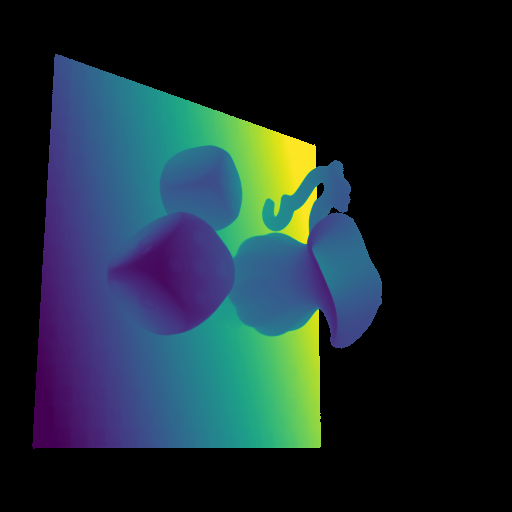
\includegraphics[width=\tw]{figures/teaser/atlas_depth.png} &
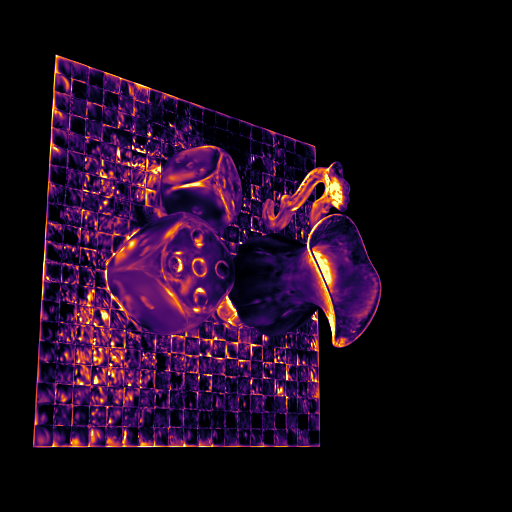
\includegraphics[width=\tw]{figures/teaser/atlas_flux.png} &
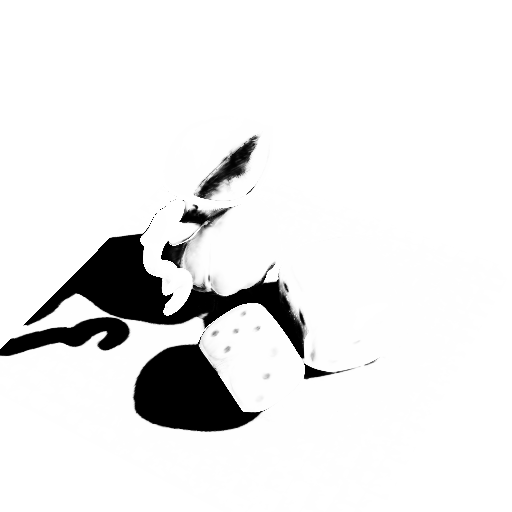
\includegraphics[width=\tw]{figures/teaser/visibility.png} &
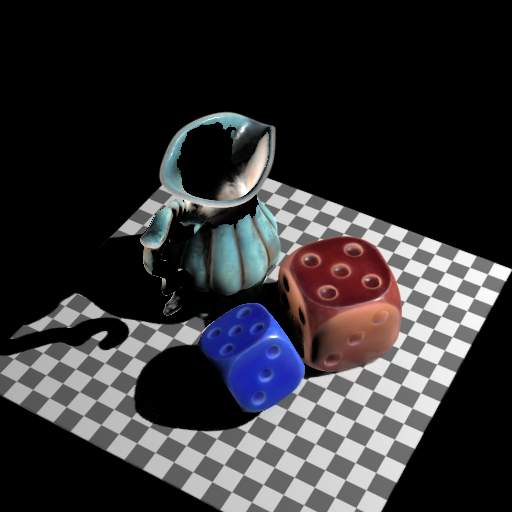
\includegraphics[width=\tw]{figures/teaser/local.png} &
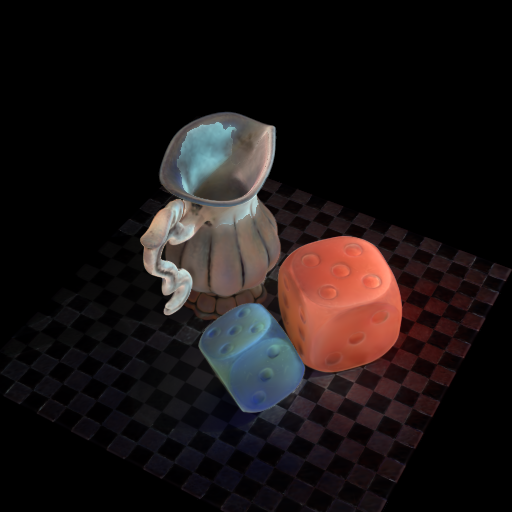
\includegraphics[width=\tw]{figures/teaser/transfer.png} &
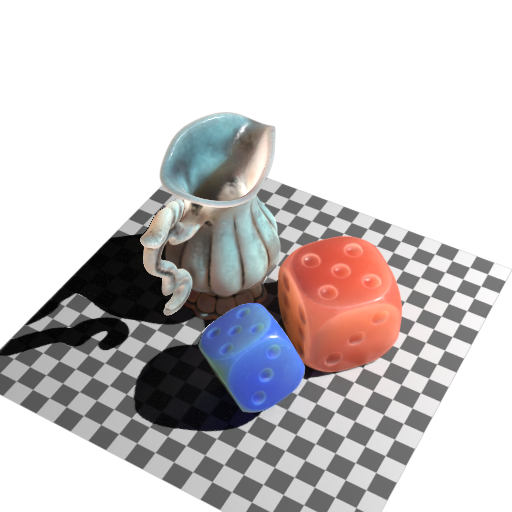
\includegraphics[width=\tw]{figures/teaser/ours.png} &
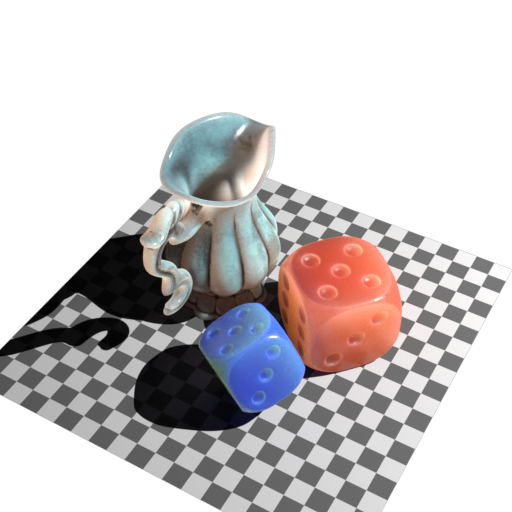
\includegraphics[width=\tw]{figures/teaser/gt.png} \\[2pt]
\small (a) atlas: depth & \small (b) atlas: flux $\boldsymbol\Phi$ & \small (c) visibility $V$ & \small (d) local term & \small (e) transfer term & \small (f) \ours & \small (g) ground truth \\
\multicolumn{2}{@{}c}{\footnotesize\textcolor{orange!70!black}{\rule[2pt]{0.06\textwidth}{0.5pt}~seen from the light~\rule[2pt]{0.06\textwidth}{0.5pt}}} &
\multicolumn{5}{c@{}}{\footnotesize\textcolor{blue!60!black}{\rule[2pt]{0.2\textwidth}{0.5pt}~seen from the camera~\rule[2pt]{0.2\textwidth}{0.5pt}}}
\end{tabular}
\captionsetup{hypcap=false}
\captionof{figure}{\textbf{Relighting from the light's point of view.}
One rasterization of the Gaussians from the point light records how deep the light is absorbed (a) and what it hits, through learned flux features (b, one of eight channels).
A camera pixel reads this atlas to decide whether it is in shadow (c) and how much light it reflects locally (d); the transfer term (e) adds radiance that the model assigns mostly to the translucent vase and dice, a learned split rather than a physical decomposition.
The sum (f) matches the test view (g) at 34.4\,dB, against 32.6\,dB for the best of four recent baselines.
Components (d, e) add in linear radiance and are shown on black.}
\captionsetup{hypcap=true}
\label{fig:teaser}
\end{strip}
